\documentclass[preprint,12pt]{elsarticle}

\usepackage{amsmath,amssymb}
\usepackage{graphicx}
\usepackage{booktabs}
\usepackage{algorithm}
\usepackage{algpseudocode}
\usepackage{hyperref}
\usepackage{float}
\usepackage{xcolor}

\journal{a journal (to be decided)}

\newcommand{\R}{\mathbb{R}}
\newcommand{\NAF}{NAF-GBLSTSVM}
\newcommand{\XX}[1]{\textcolor{red}{[#1]}}
\DeclareMathOperator*{\argmin}{arg\,min}
\newcommand{\tableorpending}[1]{\IfFileExists{tables/#1.tex}{\input{tables/#1}}{\XX{Table #1 pending: runs still in progress.}}}

\begin{document}

\begin{frontmatter}

\title{What granular-ball twin support vector machines throw away: single-sample ball deletion, label noise, tuning protocols, and a neighbour-agreement fuzzy GBLSTSVM}

% TODO before submission: confirm author names, order, affiliations and e-mail addresses.
\author[inst1]{Jayagna Patel}
\author[inst1]{[Supervisor name]}
\address[inst1]{[Department], Birla Institute of Technology and Science, Pilani, India}

\begin{abstract}
Granular-ball classifiers replace the training samples by balls produced by recursive $k$-means splitting, and are reported to be faster and more robust to label noise than their sample-based counterparts. We take a close look at one of them, the granular-ball least squares twin support vector machine (GBLSTSVM), and ask two questions: what does its ball generation actually do to noisy training data, and do its reported gains survive a strict evaluation protocol? First, GBLSTSVM deletes every ball that holds a single sample. On 35 UCI and KEEL datasets we show that this step works as a hidden noise filter that is both strong and indiscriminate: \XX{numbers from the deletion table}. Second, we treat ball memberships as detectors of mislabelled samples and find that the share of a ball's neighbours that carry its label is a far better detector than the centre-distance, entropy, overlap and density memberships used so far. This leads to a minimal fix, the neighbour-agreement fuzzy GBLSTSVM (\NAF{}), which keeps every ball and scales the error term of each ball by this agreement; training still consists of two small linear systems. Third, we compare \NAF{} with SVM, TSVM, GBSVM, LSTSVM, GBLSTSVM and LS-GBLSTSVM under two tuning protocols. When the hyperparameters are chosen by the test score, granular-ball models dominate the ranking and \NAF{} has the best average rank at every noise level, 1.2 to 1.9 points ahead of GBLSTSVM. When they are chosen by five-fold cross-validation on the training part, the ranking changes: the sample-based SVM and LSTSVM overtake GBLSTSVM at every noise level, and \NAF{} improves on GBLSTSVM mainly at high noise (3.4 points of accuracy and 4.7 points of balanced accuracy at 30\% noise). We repeat the comparison under boundary-targeted and class-dependent label noise. We conclude with recommendations for evaluating granular-ball classifiers.
\end{abstract}

\begin{keyword}
Granular-ball computing \sep Least squares twin support vector machine \sep Label noise \sep Fuzzy membership \sep Model selection \sep Evaluation protocol
\end{keyword}

\end{frontmatter}

%% ---------------------------------------------------------------------------
\section{Introduction}
\label{sec:intro}

Label noise, i.e.\ training samples that carry the wrong class label, is common in real data and harms most classifiers \cite{frenay2014}. Support vector machines (SVMs) \cite{cortes1995} are affected because a mislabelled sample near the boundary becomes a support vector with a large slack. Twin SVMs (TSVM) \cite{jayadeva2007} and least squares twin SVMs (LSTSVM) \cite{kumar2009}, which fit two non-parallel hyperplanes, share this weakness, and LSTSVM in particular uses a squared loss that grows quickly with the error of a sample.

Granular-ball computing \cite{xia2019} is a recent line of work that addresses noise and data size together. The training set is split recursively by $k$-means until every part is almost pure, each part is replaced by a ball with a centre, a radius and a majority label, and the classifier is trained on the balls. The idea has been applied to the SVM (GBSVM) \cite{xia2022gbsvm}, the twin SVM \cite{quadir2024gbtsvm} and the least squares twin SVM (GBLSTSVM and LS-GBLSTSVM) \cite{tanveer2024gblstsvm}, and fuzzy versions weight each ball by a membership \cite{xia2024gbfsvm,lang2025gbftsvm,liu2026rgbiftsvm}. The papers that introduce these models report clear gains over the sample-based models, in particular under label noise.

This paper examines GBLSTSVM closely instead of proposing yet another variant. Two observations motivated it. First, GBLSTSVM deletes every ball that holds a single sample after the splitting has ended. The usual justification is that an isolated sample is probably noise. But a correctly labelled sample also ends up alone when its closest neighbours carry the other label, which is the normal situation near the class boundary, and the boundary is exactly the region that a twin SVM needs to see. Second, the hyperparameters of granular-ball models are often chosen by the score on the test set \cite{xia2024gbfsvm,lang2025gbftsvm}, which is known to inflate the reported scores \cite{cawley2010,varma2006}, and granular-ball models have more hyperparameters than their sample-based counterparts because the ball generation adds its own.

The contributions are as follows.
\begin{enumerate}
\item \emph{Deletion analysis.} We measure on 35 datasets and under three label-noise models (uniform, boundary-targeted and class-dependent) what the deletion of single-sample balls removes. It removes most mislabelled samples, but also a large part of the correctly labelled samples, most of all the boundary and minority samples (Section~\ref{sec:deletion}).
\item \emph{Membership analysis.} We evaluate the ball memberships used in the literature as detectors of mislabelled samples and show that a vote among neighbouring balls is the only one that is clearly better than random under all three noise models (Section~\ref{sec:detection}).
\item \emph{A minimal fix.} We propose \NAF{}, which keeps every ball and weights the error term of each ball by the agreement of its neighbours. It changes GBLSTSVM in two places only and keeps its closed-form training (Section~\ref{sec:method}).
\item \emph{Protocol analysis.} We compare seven models under test-set tuning and under cross-validation (CV) tuning, and show that the protocol reverses the ranking of granular-ball and sample-based models. We report both and identify where \NAF{} helps and where it does not (Sections~\ref{sec:experiments} and \ref{sec:discussion}).
\end{enumerate}

A companion manuscript \cite{patel2026rf} builds a different membership, a radius-aware vote with a regularised formulation, on the same observation about deleted balls. The present paper is about the deletion step and the evaluation protocol themselves, and uses the simplest neighbour-based membership as the fix.

%% ---------------------------------------------------------------------------
\section{Background and related work}
\label{sec:related}

The training set is $T=\{(x_i,y_i)\}_{i=1}^{n}$ with $x_i\in\R^{d}$ and $y_i\in\{+1,-1\}$; the minority class is $+1$. $e$ is a vector of ones of suitable length.

\subsection{LSTSVM}

LSTSVM \cite{kumar2009} fits two hyperplanes $w_1^{\top}x+b_1=0$ and $w_2^{\top}x+b_2=0$. With $A$ and $B$ holding the samples of class $+1$ and $-1$ as rows, the first hyperplane solves
\begin{equation}
\min_{w_1,b_1,\xi}\ \frac{1}{2}\lVert Aw_1+eb_1\rVert^{2}+\frac{c_1}{2}\lVert\xi\rVert^{2}
\quad\text{s.t.}\quad -(Bw_1+eb_1)+\xi=e ,
\label{eq:lstsvm}
\end{equation}
so it stays close to class $+1$ and asks every sample of class $-1$ to be at distance one on the other side, with a squared penalty $\xi$ on deviations. The second hyperplane exchanges the roles of the classes. Each problem reduces to one $(d+1)\times(d+1)$ linear system. A new sample is assigned to the class of the nearer hyperplane.

\subsection{Granular balls and GBLSTSVM}

A granular ball is a group of training samples with centre $c_j=\frac{1}{n_j}\sum_{x\in GB_j}x$, radius $r_j=\frac{1}{n_j}\sum_{x\in GB_j}\lVert x-c_j\rVert$, label $y_j$ equal to the majority label, and purity equal to the share of samples that carry $y_j$ \cite{xia2019}. Generation starts from one ball holding all samples; every ball whose purity is below a threshold (0.985 here) is split by $k$-means into $k$ balls, until every ball is pure enough or holds one sample. In GBLSTSVM \cite{tanveer2024gblstsvm} the balls that hold a single sample are then deleted, and the model is trained on the centres and radii of the remaining balls. With $C^{\pm}$ the centres and $R^{\pm}$ the radii of the balls of each class, the first problem is
\begin{equation}
\min_{w_1,b_1,\xi}\ \frac{1}{2}\lVert C^{+}w_1+eb_1\rVert^{2}+\frac{c_1}{2}\lVert\xi\rVert^{2}
\quad\text{s.t.}\quad -(C^{-}w_1+eb_1)+\xi=e+R^{-} ,
\label{eq:gblstsvm}
\end{equation}
so a ball of class $-1$ must stay at distance one plus its radius. LS-GBLSTSVM adds the term $\frac{c_3}{2}(\lVert w_1\rVert^{2}+b_1^{2})$. GBSVM \cite{xia2022gbsvm} uses the ball constraint $y_j(w^{\top}c_j+b)-r_j\lVert w\rVert\ge 1-\xi_j$ in a standard SVM.

\subsection{Fuzzy memberships and noise filters}

A fuzzy SVM multiplies the penalty of each sample by a membership in $(0,1]$ \cite{lin2002}. Memberships have been computed from the distance to the class centre \cite{lin2002,batuwita2010}, from intuitionistic pairs of membership and non-membership \cite{rezvani2019}, and from the labels of the $k$ nearest neighbours, as in the fuzzy $k$-nearest-neighbour rule \cite{keller1985}. Deleting suspicious samples instead of down-weighting them is the idea of editing and filtering methods: Wilson's edited nearest neighbour rule removes samples misclassified by their neighbours \cite{wilson1972}, and classification filters remove samples misclassified by a committee \cite{brodley1999}.

On granular balls, GBFSVM \cite{xia2024gbfsvm}, GBFTSVM \cite{lang2025gbftsvm} and RGBIFTSVM \cite{liu2026rgbiftsvm} compute the membership of a ball from the distance of its centre to its class centre, the latter two also with a non-membership from the purity. The granular-ball fuzzy RVFL network of \cite{quadir2026gbfrvfl} uses the share of differently labelled balls among the $k$ nearest balls inside a non-membership degree; this is the closest prior use of the quantity that we use in \NAF{}, there in a random vector functional link network and without keeping single-sample balls. None of these works analyses what the deletion step removes, and none compares tuning protocols.

%% ---------------------------------------------------------------------------
\section{Experimental setting shared by all analyses}
\label{sec:setup}

\paragraph{Datasets} We use the 35 binary UCI \cite{uci} and KEEL \cite{keel} datasets of Table~\ref{tab:datasets}, with 80 to 1484 samples, 3 to 60 features and imbalance ratios from 1.0 to 32.7. Each dataset is split 10 times at random (5 times for the boundary-targeted and class-dependent noise) into 70\% training and 30\% test data, stratified by class; the features are standardised with the statistics of the training part. Label noise is applied to the training part only; the test labels are always clean.

\begin{table}[!t]
\centering
\caption{The 35 UCI and KEEL benchmark datasets. IR is the imbalance ratio (majority size divided by minority size).}
\label{tab:datasets}
\footnotesize
\resizebox{\textwidth}{!}{%
\begin{tabular}{lrrr@{\hskip 18pt}lrrr}
\toprule
Dataset & Samples & Features & IR & Dataset & Samples & Features & IR \\
\midrule
abalone9-18 & 731 & 7 & 16.40 & led7digit-0-2-4-5-6-7-8-9\_vs\_1 & 443 & 7 & 10.97 \\
brwisconsin & 683 & 9 & 1.86 & monk2 & 601 & 7 & 1.92 \\
bupa or liver-disorders & 345 & 6 & 1.38 & monk3 & 554 & 6 & 1.01 \\
cleve & 297 & 13 & 1.17 & new-thyroid1 & 215 & 5 & 5.14 \\
ecoli-0-1-4-6\_vs\_5 & 280 & 6 & 13.00 & pima & 768 & 8 & 1.87 \\
ecoli-0-1-4-7\_vs\_2-3-5-6 & 336 & 7 & 10.59 & sonar & 208 & 60 & 1.14 \\
ecoli-0-1\_vs\_5 & 240 & 6 & 11.00 & transfusion & 748 & 4 & 3.20 \\
ecoli2 & 336 & 7 & 8.60 & vehicle 1 & 846 & 18 & 2.90 \\
ecoli3 & 336 & 7 & 8.60 & vehicle2 & 846 & 18 & 2.88 \\
ecoli4 & 336 & 7 & 15.80 & wdbc & 569 & 30 & 1.68 \\
fertility & 100 & 9 & 7.33 & wpbc & 194 & 33 & 3.22 \\
ger & 1000 & 24 & 2.33 & yeast-0-2-5-6\_vs\_3-7-8-9 & 1004 & 8 & 9.14 \\
glass2 & 214 & 9 & 11.59 & yeast-0-2-5-7-9\_vs\_3-6-8 & 1004 & 8 & 9.14 \\
glass4 & 214 & 9 & 15.46 & yeast-0-5-6-7-9\_vs\_4 & 528 & 8 & 9.35 \\
glass5 & 214 & 9 & 22.78 & yeast-2\_vs\_4 & 514 & 8 & 9.08 \\
haberman & 306 & 3 & 2.78 & yeast1vs7 & 459 & 8 & 14.30 \\
heart-stat & 270 & 13 & 1.25 & yeast3 & 1484 & 8 & 8.10 \\
iono & 351 & 33 & 1.79 &  &  &  &  \\
\bottomrule
\end{tabular}}
\end{table}


\paragraph{Noise models} Let $q$ be the noise level.
\begin{itemize}
\item \emph{Uniform}: $\lfloor qn\rfloor$ training labels are flipped, spread over the classes in proportion to their size, with the samples chosen at random. This is the noise used in \cite{tanveer2024gblstsvm} and in most granular-ball papers; $q\in\{0.05,0.1,0.15,0.2,0.3\}$.
\item \emph{Boundary-targeted}: the same number of flips per class as uniform noise, but sample $i$ is chosen with probability proportional to $\exp(-\delta_i/\tau)$, where $\delta_i$ is its distance to the nearest training sample of the other class and $\tau$ is half the median of $\delta$ in its class. Samples close to the other class are thus flipped much more often, as when annotators confuse borderline cases.
\item \emph{Class-dependent}: a share $q$ of the majority-class samples is relabelled as minority; the minority class is untouched (noise rates $\rho_{\text{maj}}=q$, $\rho_{\text{min}}=0$ \cite{natarajan2013}).
\end{itemize}

\paragraph{Ball generation} All granular-ball models use the same generation with purity threshold 0.985 and $k\in\{2,\dots,6\}$ clusters per split, $k$ being a hyperparameter.

%% ---------------------------------------------------------------------------
\section{What the deletion of single-sample balls removes}
\label{sec:deletion}

For every dataset, noise model, noise level and split, we generated the balls on the noisy training part for $k\in\{2,4,6\}$ and recorded which samples ended up in a single-sample ball and are therefore deleted by GBLSTSVM. We split the correctly labelled samples into \emph{boundary} samples, the quarter of each class that is closest to the other class (by the true labels), and \emph{interior} samples, the remaining three quarters. Table~\ref{tab:deletion} and Figure~\ref{fig:deletion} give the results.

\tableorpending{deletion}

\begin{figure}[t]
\centering
\IfFileExists{figures/deletion.pdf}{\includegraphics[width=\textwidth]{figures/deletion.pdf}}{\XX{Figure pending.}}
\caption{Share of training samples that end up in single-sample balls and are deleted by GBLSTSVM, by group and noise model (35 datasets).}
\label{fig:deletion}
\end{figure}

\XX{Text to be written from Table~\ref{tab:deletion} once the 35-dataset diagnostics are complete. Points to make: (i) even on clean data the deletion removes X\% of the samples; (ii) under uniform noise it removes most mislabelled samples but also X\% of the correct ones, and the correct boundary samples at about Y times the rate of the interior ones; (iii) under boundary-targeted noise the filter is weaker for the mislabelled samples and removes even more correct boundary samples; (iv) under class-dependent noise the flipped majority samples form their own small balls ... ; (v) after deletion the share of noise among the remaining samples is ...}

The mechanism is simple. A sample ends up alone when the $k$-means split that would put it with samples of its own label never happens, because its region is mixed. This is the case for a mislabelled sample inside the other class, and equally for a correct sample on the boundary or a minority sample surrounded by majority samples. The deletion step cannot tell these cases apart, because it uses only the size of the ball.

%% ---------------------------------------------------------------------------
\section{Which ball membership recognises a mislabelled sample?}
\label{sec:detection}

If the deletion is to be replaced by a soft weight, the weight must be low for mislabelled samples and high for correct ones. We therefore keep all balls, give every sample the membership of its ball (or 0 if its own label differs from the ball label), and measure the area under the ROC curve (AUC) of the membership as a detector of the flipped samples; 0.5 is a random score. We compare the memberships used for granular balls so far: the distance of the ball centre to the class centre \cite{xia2024gbfsvm,lang2025gbftsvm}, one minus the label entropy of the ball, the overlap of the ball with balls of the other class, and the local density of the ball. We also include the deletion itself as a 0/1 score and, as a reference, the fuzzy $k$-NN agreement computed among samples rather than balls \cite{keller1985}.

\tableorpending{detection}

\XX{Text from Table~\ref{tab:detection}. From the 21-dataset pilot: centre distance 0.70/0.65/0.60 at 10/20/30\% uniform noise, entropy below 0.5 (a flipped sample alone in its ball has zero entropy), neighbour agreement 0.885/0.868/0.821, close to the sample-level fuzzy $k$-NN. Add the boundary-targeted and class-dependent rows.}

The reason is the same as for the deletion: a ball's own properties (size, purity, entropy, distance to its class centre) say little about whether its label is right, because a mislabelled sample forms a small, pure ball of its own. What gives it away is its surroundings: the balls around it carry the other label.

%% ---------------------------------------------------------------------------
\section{Neighbour-agreement fuzzy GBLSTSVM}
\label{sec:method}

\NAF{} makes two changes to GBLSTSVM: it keeps all balls, and it multiplies the error term of each ball by the agreement of its neighbours.

\subsection{Membership}

Let $\{(c_i,r_i,y_i,n_i)\}_{i=1}^{m}$ be all balls generated from the training set, including those with $n_i=1$, and let $N_k(i)$ be the $k$ balls whose centres are nearest to $c_i$. The agreement of ball $i$ is the share of the samples in these neighbouring balls that carry the label of ball $i$,
\begin{equation}
a_i=\frac{\sum_{j\in N_k(i)} n_j\,[y_j=y_i]}{\sum_{j\in N_k(i)} n_j}\in[0,1],
\label{eq:agree}
\end{equation}
and its membership is
\begin{equation}
s_i=\max\bigl(a_i^{\gamma},\ \varepsilon\bigr),\qquad \varepsilon=10^{-3}.
\label{eq:membership}
\end{equation}
Here $[\cdot]$ is 1 if the condition holds and 0 otherwise. Counting samples ($n_j$) rather than balls lets a large neighbouring ball weigh more than a single-sample one. The exponent $\gamma\ge 1$ sharpens the weight: with $\gamma=3$ a ball whose neighbours agree half of the time gets $0.125$ instead of $0.5$. The floor $\varepsilon$ keeps every ball in the problem. A ball inside its class has $s_i=1$, a mislabelled sample surrounded by the other class has $s_i\approx\varepsilon$, and a correct boundary ball receives an intermediate weight instead of being deleted. When every sample is its own ball, \eqref{eq:agree} is the fuzzy $k$-NN membership of \cite{keller1985}, and the model becomes a fuzzy LSTSVM on the samples (FKNN-LSTSVM in our experiments).

\subsection{Model}

Let $H=[C^{+}\ e]$ and $G=[C^{-}\ e]$ hold the centres of all balls of each class with a column of ones, $S^{\pm}=\mathrm{diag}(s^{\pm})$ their memberships, and $D^{+}=\theta I$ an optional weight of the minority class, with $\theta=1$ or $\theta=\sum_{j:y_j=-1}n_j/\sum_{j:y_j=+1}n_j$ (a hyperparameter). With $z_1=[w_1;b_1]$, the first hyperplane solves
\begin{equation}
\min_{z_1,\xi}\ \frac{1}{2}(Hz_1)^{\top}D^{+}(Hz_1)+\frac{c_1}{2}\xi^{\top}S^{-}\xi
\quad\text{s.t.}\quad -Gz_1+\xi=e+R^{-},
\label{eq:naf1}
\end{equation}
and the second
\begin{equation}
\min_{z_2,\eta}\ \frac{1}{2}(Gz_2)^{\top}(Gz_2)+\frac{c_2}{2}\eta^{\top}D^{+}S^{+}\eta
\quad\text{s.t.}\quad Hz_2+\eta=e+R^{+}.
\label{eq:naf2}
\end{equation}
The membership enters only the error terms: a ball whose label is contradicted by its neighbours may lie on the wrong side of the other class's hyperplane at almost no cost, while it still counts fully in no term that pulls a hyperplane towards its own class. Substituting the constraints and setting the gradients to zero gives
\begin{align}
z_1&=-\Bigl(G^{\top}S^{-}G+\tfrac{1}{c_1}H^{\top}D^{+}H+\delta I\Bigr)^{-1}G^{\top}S^{-}(e+R^{-}),\label{eq:sol1}\\
z_2&=\Bigl(H^{\top}D^{+}S^{+}H+\tfrac{1}{c_2}G^{\top}G+\delta I\Bigr)^{-1}H^{\top}D^{+}S^{+}(e+R^{+}),\label{eq:sol2}
\end{align}
where $\delta=10^{-4}$ is a small ridge for numerical stability, used for all least squares twin models in our code. A test sample $x$ is assigned to class $+1$ if $|w_1^{\top}x+b_1|/\lVert w_1\rVert<|w_2^{\top}x+b_2|/\lVert w_2\rVert$ and to class $-1$ otherwise. With $S^{\pm}=I$ and single-sample balls deleted, \eqref{eq:naf1}--\eqref{eq:naf2} are GBLSTSVM.

\subsection{Algorithm and cost}

\begin{algorithm}[t]
\caption{Training of \NAF{}}
\label{alg:naf}
\begin{algorithmic}[1]
\Require training set $T$; clusters per split $k_{\text{split}}$; neighbours $k$; sharpness $\gamma$; $c_1,c_2$; class weight $\theta$
\State Generate granular balls by recursive $k$-means splitting (purity threshold 0.985). Keep all balls, including single-sample ones.
\For{each ball $i$}
\State Find the $k$ nearest ball centres $N_k(i)$; compute $a_i$ by \eqref{eq:agree} and $s_i$ by \eqref{eq:membership}.
\EndFor
\State Form $H$, $G$, $S^{\pm}$, $D^{+}$, and compute $z_1$, $z_2$ by \eqref{eq:sol1}--\eqref{eq:sol2}.
\Ensure $(w_1,b_1)$, $(w_2,b_2)$.
\end{algorithmic}
\end{algorithm}

With $m$ balls in $d$ dimensions, the neighbour search costs $O(m^{2}d)$ by brute force or $O(m\log m)$ per query with a $k$-d tree in low dimension (our code switches to a tree above 1000 balls), and forming and solving the two systems costs $O(md^{2}+d^{3})$, as for GBLSTSVM. Because no ball is deleted, $m$ is larger than in GBLSTSVM; the ball generation, which is shared, dominates the run time in our experiments.

%% ---------------------------------------------------------------------------
\section{Experiments}
\label{sec:experiments}

\subsection{Models, hyperparameters and protocols}

\paragraph{Models} \NAF{} is compared with the baselines of \cite{tanveer2024gblstsvm}: SVM \cite{cortes1995}, TSVM \cite{jayadeva2007}, GBSVM \cite{xia2022gbsvm}, LSTSVM \cite{kumar2009}, GBLSTSVM and LS-GBLSTSVM \cite{tanveer2024gblstsvm}, all with the linear kernel. GBSVM, GBLSTSVM and LS-GBLSTSVM delete single-sample balls as in their original versions. GBSVM is solved to optimality as a second-order cone programme \cite{diamond2016,goulart2024}. Two further models isolate the parts of \NAF{}: GBLSTSVM with all balls kept but no membership, and FKNN-LSTSVM, i.e.\ LSTSVM on the samples with the membership \eqref{eq:agree}--\eqref{eq:membership} computed among samples.

\paragraph{Hyperparameters and their meaning} $c_1,c_2$ (LSTSVM family) and $C$ (SVM, GBSVM) weigh the error terms against the closeness or margin terms and are taken from $\{10^{-3},10^{-2},\dots,10^{3}\}$; for LS-GBLSTSVM $c_1=c_2$ and the regularisation weight $c_3=c_4$ come from the same set; TSVM uses $\{2^{-5},\dots,2^{5}\}$. $k_{\text{split}}\in\{2,\dots,6\}$ is the number of clusters per split in the ball generation. For \NAF{} and FKNN-LSTSVM, the number of neighbours is $k\in\{5,10\}$ and the sharpness $\gamma\in\{1,3\}$. Every model may switch the minority-class weight $\theta$ on or off. The number of settings searched per split is therefore 14 for SVM, 242 for TSVM, 70 for GBSVM, 98 for LSTSVM, 490 for GBLSTSVM and LS-GBLSTSVM, 392 for FKNN-LSTSVM and 1960 for \NAF{}.

\paragraph{Two tuning protocols}
\begin{itemize}
\item \emph{Test-set tuning}: for each split the reported score is the best test score over all settings. Several granular-ball papers choose their hyperparameters in this way \cite{xia2024gbfsvm,lang2025gbftsvm}. The GBLSTSVM paper states five-fold CV \cite{tanveer2024gblstsvm}; on the datasets we share with it, our test-tuned scores of GBLSTSVM are close to the published ones and our CV-tuned scores are several points lower.
\item \emph{CV tuning}: the setting with the best mean balanced accuracy in five-fold CV on the (noisy) training part is chosen, the model is retrained on the whole training part and scored once on the test part. This is what a user can do in practice.
\end{itemize}

\paragraph{Scores and tests} We report accuracy (ACC) and balanced accuracy (BACC, the mean recall of the two classes) in per cent, averaged over the splits of each dataset. Models are compared by their average rank over the datasets with the Friedman test and the Iman--Davenport correction \cite{demsar2006,iman1980} (Table~\ref{tab:friedman}), and \NAF{} is compared with every other model by the Wilcoxon signed-rank test and win/tie/loss counts over the 35 datasets.

\subsection{Uniform noise, test-set tuning}

Table~\ref{tab:uni-oracle} gives the average ACC and rank. Under this protocol the three granular-ball least squares models occupy the first places. \NAF{} has the best average rank at every noise level (1.6 to 2.1). Its average ACC is the same as that of LS-GBLSTSVM to within 0.05 points (89.5\% on clean data, 88.7\% at 20\% noise, 87.5\% at 30\%), and the difference between the two is not significant at any level (Table~\ref{tab:uni-oracle-pair}). \NAF{} is 1.2 to 1.9 points ahead of GBLSTSVM, which it modifies, with 27 to 31 wins out of 35 ($p<0.001$ at every level), and 0.7 to 2.5 points ahead of SVM, TSVM and LSTSVM ($p<0.001$). Keeping the balls without a membership already gives part of the gain; the membership adds a further 0.6 to 1.4 points ($p<0.001$). \NAF{} is also 0.6 to 0.8 points ahead of FKNN-LSTSVM.

\begin{table}[!t]
\centering
\caption{Uniform label noise, test-set tuning: average ACC (\%) and average rank over 35 datasets (10 splits). Best value in each row in bold.}
\label{tab:uni-oracle}
\small
\resizebox{\textwidth}{!}{%
\begin{tabular}{llccccccc}
\toprule
 & Noise & SVM & TSVM & GBSVM & LSTSVM & GBLSTSVM & LS-GBLSTSVM & \textbf{NAF-GBLSTSVM} \\
\midrule
Average ACC & 0\% & 88.53 & 88.59 & 84.96 & 88.21 & 88.08 & \textbf{89.50} & \textbf{89.50} \\
 & 5\% & 87.91 & 88.61 & 85.11 & 88.05 & 87.98 & \textbf{89.30} & \textbf{89.30} \\
 & 10\% & 87.08 & 88.23 & 84.87 & 87.56 & 87.93 & \textbf{89.20} & 89.16 \\
 & 15\% & 86.47 & 87.59 & 84.58 & 87.14 & 87.52 & 88.87 & \textbf{88.90} \\
 & 20\% & 86.17 & 87.07 & 83.97 & 86.79 & 87.06 & 88.66 & \textbf{88.67} \\
 & 30\% & 85.39 & 85.33 & 83.09 & 85.27 & 85.56 & 87.41 & \textbf{87.46} \\
\midrule
Average rank & 0\% & 4.81 & 4.16 & 5.40 & 5.23 & 4.07 & 2.24 & \textbf{2.09} \\
 & 5\% & 5.31 & 3.90 & 5.27 & 5.44 & 3.83 & 2.30 & \textbf{1.94} \\
 & 10\% & 5.53 & 4.16 & 5.17 & 5.44 & 3.87 & 1.99 & \textbf{1.84} \\
 & 15\% & 5.61 & 4.31 & 5.51 & 5.31 & 3.49 & 2.14 & \textbf{1.61} \\
 & 20\% & 5.63 & 4.37 & 5.67 & 5.00 & 3.54 & 2.06 & \textbf{1.73} \\
 & 30\% & 5.37 & 4.70 & 5.81 & 4.69 & 3.56 & 2.06 & \textbf{1.81} \\
\bottomrule
\end{tabular}}
\end{table}

\begin{table}[!t]
\centering
\caption{NAF-GBLSTSVM against each other model, uniform noise, test-set tuning: mean difference in ACC (points; positive = NAF-GBLSTSVM better), [win, tie, loss] over the 35 datasets and, in parentheses, the $p$-value of the Wilcoxon signed-rank test.}
\label{tab:uni-oracle-pair}
\footnotesize
\resizebox{\textwidth}{!}{%
\begin{tabular}{lcccccc}
\toprule
Compared model & 0\% & 5\% & 10\% & 15\% & 20\% & 30\% \\
\midrule
SVM & \shortstack{+0.97 [29, 1, 5]\\($<$0.001)} & \shortstack{+1.39 [30, 0, 5]\\($<$0.001)} & \shortstack{+2.08 [33, 0, 2]\\($<$0.001)} & \shortstack{+2.43 [33, 0, 2]\\($<$0.001)} & \shortstack{+2.49 [34, 0, 1]\\($<$0.001)} & \shortstack{+2.07 [32, 1, 2]\\($<$0.001)} \\[4pt]
TSVM & \shortstack{+0.91 [29, 0, 6]\\($<$0.001)} & \shortstack{+0.69 [31, 0, 4]\\($<$0.001)} & \shortstack{+0.92 [32, 1, 2]\\($<$0.001)} & \shortstack{+1.31 [33, 0, 2]\\($<$0.001)} & \shortstack{+1.60 [34, 0, 1]\\($<$0.001)} & \shortstack{+2.13 [33, 1, 1]\\($<$0.001)} \\[4pt]
GBSVM & \shortstack{+4.55 [33, 0, 2]\\($<$0.001)} & \shortstack{+4.19 [31, 1, 3]\\($<$0.001)} & \shortstack{+4.29 [30, 0, 5]\\($<$0.001)} & \shortstack{+4.32 [33, 0, 2]\\($<$0.001)} & \shortstack{+4.70 [32, 2, 1]\\($<$0.001)} & \shortstack{+4.37 [31, 1, 3]\\($<$0.001)} \\[4pt]
LSTSVM & \shortstack{+1.29 [32, 0, 3]\\($<$0.001)} & \shortstack{+1.25 [32, 1, 2]\\($<$0.001)} & \shortstack{+1.60 [34, 0, 1]\\($<$0.001)} & \shortstack{+1.76 [35, 0, 0]\\($<$0.001)} & \shortstack{+1.87 [35, 0, 0]\\($<$0.001)} & \shortstack{+2.19 [34, 1, 0]\\($<$0.001)} \\[4pt]
GBLSTSVM & \shortstack{+1.42 [27, 4, 4]\\($<$0.001)} & \shortstack{+1.33 [30, 0, 5]\\($<$0.001)} & \shortstack{+1.22 [30, 2, 3]\\($<$0.001)} & \shortstack{+1.37 [31, 0, 4]\\($<$0.001)} & \shortstack{+1.60 [27, 3, 5]\\($<$0.001)} & \shortstack{+1.90 [28, 2, 5]\\($<$0.001)} \\[4pt]
LS-GBLSTSVM & \shortstack{-0.00 [19, 1, 15]\\(0.289)} & \shortstack{-0.00 [21, 2, 12]\\(0.140)} & \shortstack{-0.05 [18, 4, 13]\\(0.451)} & \shortstack{+0.03 [22, 3, 10]\\(0.172)} & \shortstack{+0.01 [19, 2, 14]\\(0.649)} & \shortstack{+0.05 [20, 1, 14]\\(0.632)} \\[4pt]
GBLSTSVM, all balls kept & \shortstack{+0.56 [31, 0, 4]\\($<$0.001)} & \shortstack{+0.86 [34, 0, 1]\\($<$0.001)} & \shortstack{+0.89 [35, 0, 0]\\($<$0.001)} & \shortstack{+0.97 [34, 0, 1]\\($<$0.001)} & \shortstack{+1.18 [32, 1, 2]\\($<$0.001)} & \shortstack{+1.38 [32, 2, 1]\\($<$0.001)} \\[4pt]
FKNN-LSTSVM & \shortstack{+0.63 [30, 1, 4]\\($<$0.001)} & \shortstack{+0.60 [29, 1, 5]\\($<$0.001)} & \shortstack{+0.61 [29, 0, 6]\\($<$0.001)} & \shortstack{+0.63 [31, 0, 4]\\($<$0.001)} & \shortstack{+0.72 [32, 0, 3]\\($<$0.001)} & \shortstack{+0.82 [30, 1, 4]\\($<$0.001)} \\[4pt]
\bottomrule
\end{tabular}}
\end{table}


\subsection{Uniform noise, CV tuning}

Tables~\ref{tab:uni-cv-acc}--\ref{tab:uni-cv-bacc-pair} give the results under CV tuning. All scores drop, by 5 to 30 points, and the order changes.

\emph{Accuracy.} On clean data SVM is best (83.2\%), followed by TSVM, LS-GBLSTSVM and LSTSVM (81.0 to 81.9\%); \NAF{} reaches 79.0\% and GBLSTSVM 78.2\%. LS-GBLSTSVM is the strongest model from 5\% to 20\% noise. Against GBLSTSVM, \NAF{} is level up to 10\% noise and ahead from 15\% upwards, by 1.3, 2.1 and 3.4 points at 15\%, 20\% and 30\% ($p=0.18$, $0.027$, $0.007$). At 30\% noise it is ahead of LSTSVM (67.5\% against 66.0\%) and TSVM, but behind SVM (72.2\%) and LS-GBLSTSVM (70.0\%).

\emph{Balanced accuracy.} Here \NAF{} improves on GBLSTSVM at every noise level, by 2.5 points on clean data and 4.7 points at 30\% noise ($p<0.001$ for both), because the deleted single-sample balls belong disproportionately to the minority class. It is level with LS-GBLSTSVM (no significant difference except at 5\% noise) and behind SVM, TSVM and LSTSVM up to 20\% noise, by 1.2 to 4.4 points; at 30\% noise these differences are no longer significant.

\XX{FKNN-LSTSVM under CV tuning: pending (results/paper\_cv\_fknn).}

\begin{table}[!t]
\centering
\caption{Uniform label noise, cross-validated tuning: average ACC (\%) and average rank over 35 datasets (10 splits).}
\label{tab:uni-cv-acc}
\small
\resizebox{\textwidth}{!}{%
\begin{tabular}{llccccccc}
\toprule
 & Noise & SVM & TSVM & GBSVM & LSTSVM & GBLSTSVM & LS-GBLSTSVM & \textbf{NAF-GBLSTSVM} \\
\midrule
Average ACC & 0\% & \textbf{83.22} & 81.92 & 68.56 & 81.01 & 78.23 & 81.45 & 79.03 \\
 & 5\% & 79.76 & 79.11 & 70.26 & 79.41 & 77.77 & \textbf{81.10} & 77.44 \\
 & 10\% & 77.82 & 77.74 & 68.74 & 77.47 & 76.40 & \textbf{80.01} & 76.38 \\
 & 15\% & 75.98 & 74.99 & 64.15 & 75.82 & 74.32 & \textbf{77.47} & 75.61 \\
 & 20\% & 74.42 & 73.14 & 61.26 & 73.46 & 70.49 & \textbf{75.13} & 72.63 \\
 & 30\% & \textbf{72.20} & 65.52 & 52.50 & 66.05 & 64.06 & 70.03 & 67.48 \\
\midrule
Average rank & 0\% & \textbf{2.63} & 3.27 & 5.63 & 3.66 & 4.81 & 3.41 & 4.59 \\
 & 5\% & 3.53 & 3.63 & 5.54 & 3.40 & 4.80 & \textbf{2.61} & 4.49 \\
 & 10\% & 3.63 & 3.36 & 5.57 & 3.60 & 4.83 & \textbf{2.79} & 4.23 \\
 & 15\% & 3.73 & 3.99 & 5.34 & 3.44 & 4.66 & \textbf{2.91} & 3.93 \\
 & 20\% & 3.10 & 3.63 & 5.71 & 3.47 & 4.91 & \textbf{3.07} & 4.10 \\
 & 30\% & \textbf{2.26} & 3.99 & 5.89 & 4.24 & 4.77 & 3.10 & 3.76 \\
\bottomrule
\end{tabular}}
\end{table}

\begin{table}[!t]
\centering
\caption{NAF-GBLSTSVM against each other model, uniform noise, cross-validated tuning: mean difference in ACC (points; positive = NAF-GBLSTSVM better), [win, tie, loss] over the 35 datasets and, in parentheses, the $p$-value of the Wilcoxon signed-rank test.}
\label{tab:uni-cv-acc-pair}
\footnotesize
\resizebox{\textwidth}{!}{%
\begin{tabular}{lcccccc}
\toprule
Compared model & 0\% & 5\% & 10\% & 15\% & 20\% & 30\% \\
\midrule
SVM & \shortstack{-4.18 [5, 0, 30]\\($<$0.001)} & \shortstack{-2.32 [14, 0, 21]\\(0.055)} & \shortstack{-1.44 [15, 0, 20]\\(0.342)} & \shortstack{-0.36 [17, 0, 18]\\(0.743)} & \shortstack{-1.79 [12, 0, 23]\\(0.199)} & \shortstack{-4.72 [9, 0, 26]\\(0.001)} \\[4pt]
TSVM & \shortstack{-2.88 [11, 1, 23]\\(0.003)} & \shortstack{-1.67 [12, 0, 23]\\(0.047)} & \shortstack{-1.35 [14, 0, 21]\\(0.072)} & \shortstack{+0.62 [18, 2, 15]\\(0.823)} & \shortstack{-0.51 [15, 0, 20]\\(0.132)} & \shortstack{+1.97 [18, 0, 17]\\(0.225)} \\[4pt]
GBSVM & \shortstack{+10.47 [27, 0, 8]\\($<$0.001)} & \shortstack{+7.18 [26, 0, 9]\\(0.003)} & \shortstack{+7.64 [26, 0, 9]\\(0.002)} & \shortstack{+11.47 [27, 0, 8]\\($<$0.001)} & \shortstack{+11.37 [26, 0, 9]\\($<$0.001)} & \shortstack{+14.98 [28, 0, 7]\\($<$0.001)} \\[4pt]
LSTSVM & \shortstack{-1.98 [11, 0, 24]\\(0.018)} & \shortstack{-1.96 [10, 0, 25]\\(0.010)} & \shortstack{-1.09 [11, 0, 24]\\(0.132)} & \shortstack{-0.21 [12, 0, 23]\\(0.101)} & \shortstack{-0.83 [16, 1, 18]\\(0.326)} & \shortstack{+1.43 [21, 0, 14]\\(0.100)} \\[4pt]
GBLSTSVM & \shortstack{+0.80 [21, 0, 14]\\(0.310)} & \shortstack{-0.33 [17, 0, 18]\\(0.974)} & \shortstack{-0.02 [21, 1, 13]\\(0.688)} & \shortstack{+1.30 [21, 1, 13]\\(0.180)} & \shortstack{+2.14 [22, 0, 13]\\(0.027)} & \shortstack{+3.42 [24, 0, 11]\\(0.007)} \\[4pt]
LS-GBLSTSVM & \shortstack{-2.42 [9, 0, 26]\\(0.004)} & \shortstack{-3.65 [9, 0, 26]\\(0.001)} & \shortstack{-3.63 [9, 1, 25]\\(0.002)} & \shortstack{-1.86 [11, 0, 24]\\(0.022)} & \shortstack{-2.50 [10, 0, 25]\\(0.013)} & \shortstack{-2.55 [13, 1, 21]\\(0.144)} \\[4pt]
GBLSTSVM, all balls kept & \shortstack{-0.69 [18, 0, 17]\\(0.422)} & \shortstack{+0.73 [21, 1, 13]\\(0.086)} & \shortstack{-0.30 [16, 0, 19]\\(0.909)} & \shortstack{+1.13 [21, 1, 13]\\(0.122)} & \shortstack{+0.89 [21, 0, 14]\\(0.258)} & \shortstack{+2.51 [23, 1, 11]\\(0.018)} \\[4pt]
FKNN-LSTSVM & -- & -- & -- & -- & -- & -- \\[4pt]
\bottomrule
\end{tabular}}
\end{table}

\begin{table}[!t]
\centering
\caption{Uniform label noise, cross-validated tuning: average balanced accuracy (BACC, \%) and average rank over 35 datasets.}
\label{tab:uni-cv-bacc}
\small
\resizebox{\textwidth}{!}{%
\begin{tabular}{llccccccc}
\toprule
 & Noise & SVM & TSVM & GBSVM & LSTSVM & GBLSTSVM & LS-GBLSTSVM & \textbf{NAF-GBLSTSVM} \\
\midrule
Average BACC & 0\% & \textbf{81.01} & 80.32 & 66.99 & 80.45 & 74.17 & 76.93 & 76.62 \\
 & 5\% & \textbf{79.79} & 78.68 & 69.85 & 79.20 & 75.11 & 77.83 & 76.70 \\
 & 10\% & \textbf{78.75} & 77.87 & 69.24 & 77.93 & 74.15 & 76.48 & 75.43 \\
 & 15\% & \textbf{76.85} & 75.46 & 67.44 & 76.37 & 72.33 & 74.59 & 74.22 \\
 & 20\% & \textbf{75.21} & 74.53 & 65.56 & 74.32 & 69.99 & 72.85 & 72.77 \\
 & 30\% & \textbf{69.72} & 68.56 & 59.65 & 68.69 & 63.68 & 67.96 & 68.43 \\
\midrule
Average rank & 0\% & \textbf{2.29} & 2.47 & 6.29 & 2.64 & 5.54 & 4.43 & 4.34 \\
 & 5\% & \textbf{2.53} & 3.37 & 5.89 & 2.81 & 5.31 & 3.57 & 4.51 \\
 & 10\% & \textbf{2.60} & 2.94 & 5.79 & 2.76 & 5.11 & 3.97 & 4.83 \\
 & 15\% & \textbf{2.57} & 3.60 & 5.71 & 2.66 & 5.17 & 4.09 & 4.20 \\
 & 20\% & \textbf{2.43} & 2.77 & 5.97 & 2.99 & 5.49 & 4.11 & 4.24 \\
 & 30\% & \textbf{2.97} & 3.17 & 5.71 & 3.43 & 5.23 & 4.00 & 3.49 \\
\bottomrule
\end{tabular}}
\end{table}

\begin{table}[!t]
\centering
\caption{NAF-GBLSTSVM against each other model, uniform noise, cross-validated tuning: mean difference in BACC (points; positive = NAF-GBLSTSVM better), [win, tie, loss] over the 35 datasets and, in parentheses, the $p$-value of the Wilcoxon signed-rank test.}
\label{tab:uni-cv-bacc-pair}
\footnotesize
\resizebox{\textwidth}{!}{%
\begin{tabular}{lcccccc}
\toprule
Compared model & 0\% & 5\% & 10\% & 15\% & 20\% & 30\% \\
\midrule
SVM & \shortstack{-4.38 [5, 0, 30]\\($<$0.001)} & \shortstack{-3.09 [9, 0, 26]\\($<$0.001)} & \shortstack{-3.31 [6, 0, 29]\\($<$0.001)} & \shortstack{-2.63 [10, 0, 25]\\($<$0.001)} & \shortstack{-2.45 [9, 0, 26]\\($<$0.001)} & \shortstack{-1.29 [14, 0, 21]\\(0.201)} \\[4pt]
TSVM & \shortstack{-3.70 [6, 0, 29]\\($<$0.001)} & \shortstack{-1.98 [9, 0, 26]\\($<$0.001)} & \shortstack{-2.44 [7, 0, 28]\\($<$0.001)} & \shortstack{-1.24 [13, 0, 22]\\(0.025)} & \shortstack{-1.77 [7, 0, 28]\\($<$0.001)} & \shortstack{-0.13 [14, 0, 21]\\(0.201)} \\[4pt]
GBSVM & \shortstack{+9.63 [31, 0, 4]\\($<$0.001)} & \shortstack{+6.85 [26, 0, 9]\\($<$0.001)} & \shortstack{+6.19 [26, 0, 9]\\(0.001)} & \shortstack{+6.78 [25, 0, 10]\\($<$0.001)} & \shortstack{+7.21 [28, 0, 7]\\($<$0.001)} & \shortstack{+8.78 [28, 0, 7]\\($<$0.001)} \\[4pt]
LSTSVM & \shortstack{-3.83 [4, 0, 31]\\($<$0.001)} & \shortstack{-2.50 [8, 0, 27]\\($<$0.001)} & \shortstack{-2.50 [4, 0, 31]\\($<$0.001)} & \shortstack{-2.15 [8, 0, 27]\\($<$0.001)} & \shortstack{-1.55 [8, 1, 26]\\($<$0.001)} & \shortstack{-0.26 [17, 0, 18]\\(0.461)} \\[4pt]
GBLSTSVM & \shortstack{+2.45 [30, 0, 5]\\($<$0.001)} & \shortstack{+1.59 [24, 0, 11]\\(0.035)} & \shortstack{+1.28 [19, 0, 16]\\(0.145)} & \shortstack{+1.89 [23, 0, 12]\\(0.026)} & \shortstack{+2.78 [27, 0, 8]\\($<$0.001)} & \shortstack{+4.74 [30, 0, 5]\\($<$0.001)} \\[4pt]
LS-GBLSTSVM & \shortstack{-0.31 [17, 0, 18]\\(0.974)} & \shortstack{-1.14 [11, 0, 24]\\(0.036)} & \shortstack{-1.05 [14, 0, 21]\\(0.201)} & \shortstack{-0.37 [19, 0, 16]\\(0.831)} & \shortstack{-0.08 [17, 0, 18]\\(0.781)} & \shortstack{+0.46 [20, 0, 15]\\(0.578)} \\[4pt]
GBLSTSVM, all balls kept & \shortstack{-0.26 [14, 0, 21]\\(0.481)} & \shortstack{+0.81 [21, 0, 14]\\(0.287)} & \shortstack{+0.16 [18, 0, 17]\\(0.831)} & \shortstack{+0.87 [23, 0, 12]\\(0.074)} & \shortstack{+0.94 [21, 0, 14]\\(0.112)} & \shortstack{+2.73 [27, 0, 8]\\($<$0.001)} \\[4pt]
FKNN-LSTSVM & -- & -- & -- & -- & -- & -- \\[4pt]
\bottomrule
\end{tabular}}
\end{table}


\begin{figure}[t]
\centering
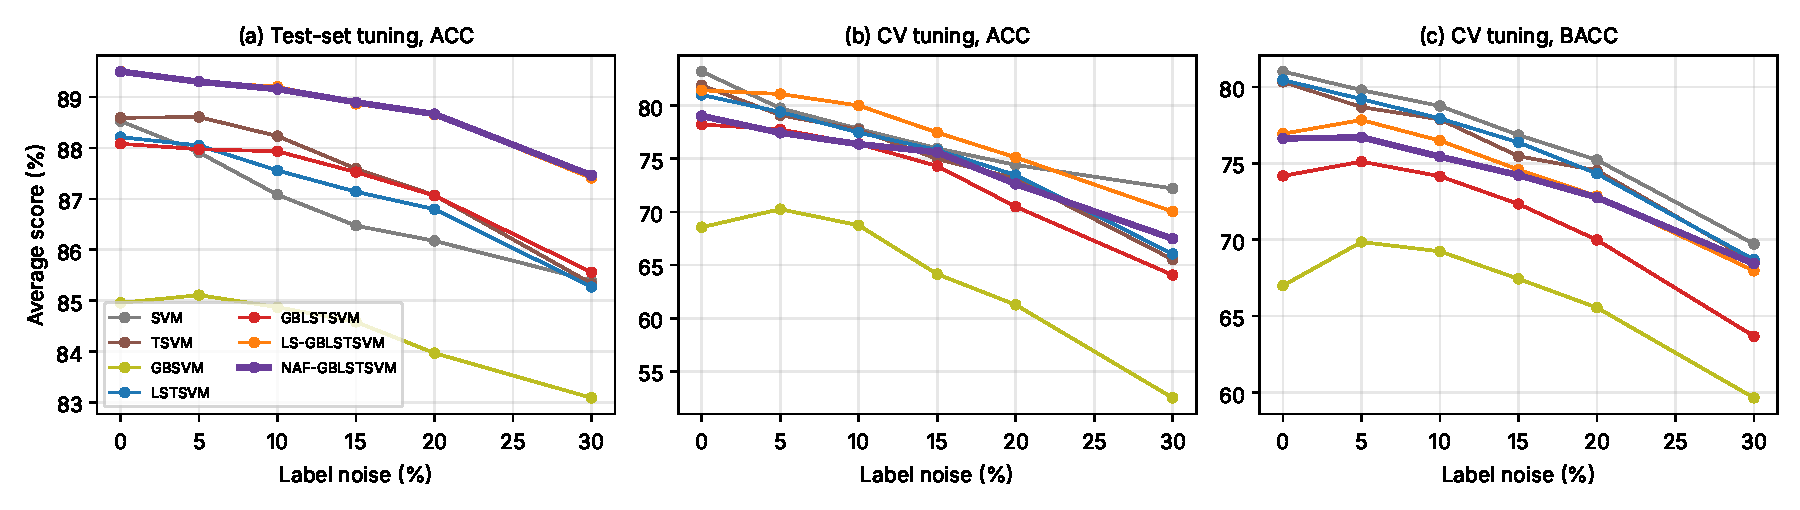
\includegraphics[width=\textwidth]{figures/noise_uniform.pdf}
\caption{Uniform noise: average score over 35 datasets against the noise level under the two protocols.}
\label{fig:noise-uniform}
\end{figure}

\subsection{How much the protocol matters}

Table~\ref{tab:protocol} and Figure~\ref{fig:protocol} put the two protocols side by side. Every model gains from test-set tuning, but not equally. On clean data, SVM gains 5.3 points of ACC, LSTSVM 7.2, GBLSTSVM 9.9 and \NAF{} 10.5; GBSVM gains 16.4. The gain grows with the noise level and is larger for the granular-ball least squares models, which search five times more settings than LSTSVM, than for SVM, TSVM and LSTSVM. (GBSVM is a special case: under CV tuning its exact solution often collapses to one class, see \cite{patel2026rf}.) As a result, the ranks change: on clean data, GBLSTSVM is ranked above SVM, TSVM and LSTSVM under test-set tuning (4.1 against 4.8, 4.2 and 5.2) and below all three under CV tuning (4.8 against 2.6, 3.3 and 3.7), and the same reversal holds at 10\%, 20\% and 30\% noise. \NAF{} drops from rank 2.1 to 4.6 on clean data and from 1.8 to 3.8 at 30\% noise. A claim that a granular-ball model beats a sample-based one therefore depends on the protocol, and test-set tuning favours the models with more hyperparameters.

\begin{table}[!t]
\centering
\caption{How much each model gains when its hyperparameters are chosen on the test set instead of by cross-validation on the training part (linear kernel, uniform noise, 35 datasets). Gap: average test-tuned ACC minus average CV-tuned ACC, in points. Rank: average rank among the seven models under test-set tuning $\to$ under CV tuning. Settings: number of hyperparameter combinations searched per split.}
\label{tab:protocol}
\small
\resizebox{\textwidth}{!}{%
\begin{tabular}{lrcccccccc}
\toprule
 & & \multicolumn{2}{c}{0\% noise} & \multicolumn{2}{c}{10\% noise} & \multicolumn{2}{c}{20\% noise} & \multicolumn{2}{c}{30\% noise} \\
\cmidrule(lr){3-4} \cmidrule(lr){5-6} \cmidrule(lr){7-8} \cmidrule(lr){9-10}
Model & Settings & Gap & Rank & Gap & Rank & Gap & Rank & Gap & Rank \\
\midrule
SVM & 14 & 5.3 & 4.8 $\to$ 2.6 & 9.3 & 5.5 $\to$ 3.6 & 11.7 & 5.6 $\to$ 3.1 & 13.2 & 5.4 $\to$ 2.3 \\
TSVM & 242 & 6.7 & 4.2 $\to$ 3.3 & 10.5 & 4.2 $\to$ 3.4 & 13.9 & 4.4 $\to$ 3.6 & 19.8 & 4.7 $\to$ 4.0 \\
GBSVM & 70 & 16.4 & 5.4 $\to$ 5.6 & 16.1 & 5.2 $\to$ 5.6 & 22.7 & 5.7 $\to$ 5.7 & 30.6 & 5.8 $\to$ 5.9 \\
LSTSVM & 98 & 7.2 & 5.2 $\to$ 3.7 & 10.1 & 5.4 $\to$ 3.6 & 13.3 & 5.0 $\to$ 3.5 & 19.2 & 4.7 $\to$ 4.2 \\
GBLSTSVM & 490 & 9.9 & 4.1 $\to$ 4.8 & 11.5 & 3.9 $\to$ 4.8 & 16.6 & 3.5 $\to$ 4.9 & 21.5 & 3.6 $\to$ 4.8 \\
LS-GBLSTSVM & 490 & 8.1 & 2.2 $\to$ 3.4 & 9.2 & 2.0 $\to$ 2.8 & 13.5 & 2.1 $\to$ 3.1 & 17.4 & 2.1 $\to$ 3.1 \\
\textbf{NAF-GBLSTSVM} & 1960 & 10.5 & 2.1 $\to$ 4.6 & 12.8 & 1.8 $\to$ 4.2 & 16.0 & 1.7 $\to$ 4.1 & 20.0 & 1.8 $\to$ 3.8 \\
\bottomrule
\end{tabular}}
\end{table}


\begin{figure}[t]
\centering
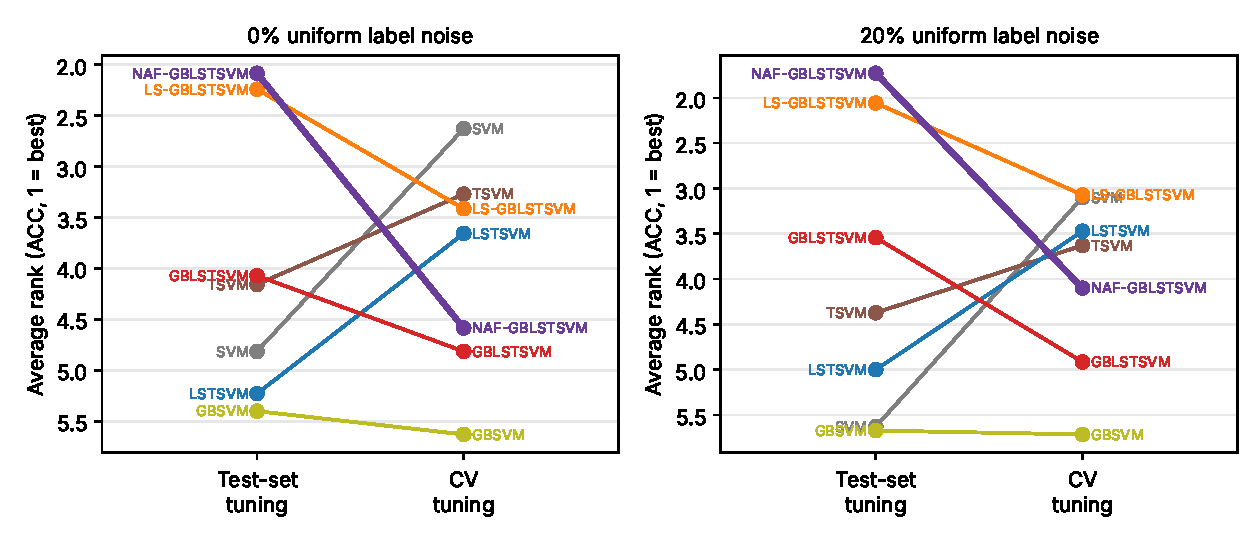
\includegraphics[width=0.9\textwidth]{figures/protocol.pdf}
\caption{Average rank (ACC) of the seven models under test-set tuning and CV tuning on the same splits.}
\label{fig:protocol}
\end{figure}

\subsection{Where the gain comes from}

Table~\ref{tab:ablation} separates keeping the balls from weighting them. \XX{Text: keeping all balls ... ; adding the membership ... ; FKNN-LSTSVM ...}

\begin{table}[!t]
\centering
\caption{Where the gain of NAF-GBLSTSVM comes from (linear kernel, uniform noise, average ACC in \% over 35 datasets). The last two rows train on the samples instead of the balls; FKNN-LSTSVM gives every sample the neighbour-agreement membership of \eqref{eq:agree} computed among samples, i.e.\ NAF-GBLSTSVM with every sample as its own ball.}
\label{tab:ablation}
\small
\resizebox{\textwidth}{!}{%
\begin{tabular}{llcccccccc}
\toprule
 & & \multicolumn{4}{c}{Test-set tuning} & \multicolumn{4}{c}{CV tuning} \\ \cmidrule(lr){3-6}\cmidrule(lr){7-10}
Model & Trained on & 0\% & 10\% & 20\% & 30\% & 0\% & 10\% & 20\% & 30\% \\
\midrule
GBLSTSVM & balls, single-sample balls deleted & 88.08 & 87.93 & 87.06 & 85.56 & 78.23 & 76.40 & 70.49 & 64.06 \\
GBLSTSVM, all balls kept & balls, all kept & 88.95 & 88.27 & 87.49 & 86.08 & 79.72 & 76.68 & 71.74 & 64.97 \\
NAF-GBLSTSVM & balls, all kept, NAF membership & 89.50 & 89.16 & 88.67 & 87.46 & 79.03 & 76.38 & 72.63 & 67.48 \\
LSTSVM & samples & 88.21 & 87.56 & 86.79 & 85.27 & 81.01 & 77.47 & 73.46 & 66.05 \\
FKNN-LSTSVM & samples, fuzzy $k$-NN membership & 88.87 & 88.54 & 87.94 & 86.64 & -- & -- & -- & -- \\
\bottomrule
\end{tabular}}
\end{table}


\subsection{Boundary-targeted and class-dependent noise}

\tableorpending{noisetypes}

\XX{Text from Table~\ref{tab:noisetypes} and the pairwise tables (results/noise\_boundary, results/noise\_asymmetric).}

\begin{table}[!t]
\centering
\caption{Friedman test over the seven models (35 datasets). $\chi^2_F$ has 6 degrees of freedom; $F_F$ is the Iman--Davenport statistic.}
\label{tab:friedman}
\small
\begin{tabular}{lllccc}
\toprule
Noise model & Tuning & Level & $\chi^2_F$ & $F_F$ & $p$ \\
\midrule
Uniform & Test set & 0\% & 81.86 & 21.72 & $<$0.001 \\
Uniform & Test set & 10\% & 109.07 & 36.74 & $<$0.001 \\
Uniform & Test set & 20\% & 117.95 & 43.57 & $<$0.001 \\
Uniform & Test set & 30\% & 111.61 & 38.57 & $<$0.001 \\
Uniform & CV & 0\% & 48.98 & 10.34 & $<$0.001 \\
Uniform & CV & 10\% & 40.45 & 8.11 & $<$0.001 \\
Uniform & CV & 20\% & 44.06 & 9.03 & $<$0.001 \\
Uniform & CV & 30\% & 60.88 & 13.88 & $<$0.001 \\
\bottomrule
\end{tabular}
\end{table}


%% ---------------------------------------------------------------------------
\section{Discussion}
\label{sec:discussion}

\paragraph{The deletion step is a noise filter, and a blunt one} \XX{summarise Section~\ref{sec:deletion}.} Filters that delete samples misclassified by their neighbours have a long history \cite{wilson1972,brodley1999}; the deletion of single-sample balls is a filter of this kind that looks only at the size of the ball, and it pays for its noise removal with a large share of the boundary and minority samples. Replacing it by a weight that looks at the neighbours keeps those samples in the problem.

\paragraph{When to use \NAF{}} Under test-set tuning, \NAF{} is the best-ranked of the seven models at every uniform noise level, level with LS-GBLSTSVM in mean ACC. Under CV tuning its gains over GBLSTSVM appear in balanced accuracy at every noise level and in accuracy from 15\% noise upwards; on clean or mildly noisy data the sample-based SVM, TSVM and LSTSVM and the regularised LS-GBLSTSVM are better choices. \NAF{} has more hyperparameters than GBLSTSVM; with CV tuning this costs four times more fits, but each fit is still two small linear systems, and the ball generation, which dominates the time, is shared.

\paragraph{Recommendations for evaluating granular-ball classifiers} (i) Choose hyperparameters without the test labels, e.g.\ by CV on the training part, and state the protocol. (ii) Report the number of settings searched per model, since test-set tuning rewards larger grids. (iii) Include the sample-based counterpart (here LSTSVM) and a fuzzy $k$-NN version of it as baselines. (iv) Report balanced accuracy on imbalanced data. (v) Test more than uniform label noise.

\paragraph{Limitations} All experiments use the linear kernel and binary datasets with at most 1484 samples. The boundary-targeted and class-dependent noise experiments use 5 splits instead of 10. The noise models are synthetic. The neighbour search uses centre distances; the companion work \cite{patel2026rf} studies a radius-aware alternative.

%% ---------------------------------------------------------------------------
\section{Conclusion}
\label{sec:conclusion}

We examined GBLSTSVM under label noise. Its deletion of single-sample balls removes most mislabelled samples, but also many correct boundary and minority samples. Of the ball memberships in use, only a vote among neighbouring balls recognises mislabelled samples well. Keeping all balls and weighting each by this vote gives \NAF{}, a two-line change to GBLSTSVM that keeps its closed-form training. Whether \NAF{}, or any granular-ball model, beats the sample-based models depends on the tuning protocol: under test-set tuning the granular-ball models lead, under CV tuning the sample-based ones lead on clean data and \NAF{} improves on GBLSTSVM mainly at higher noise. We recommend that granular-ball classifiers be evaluated with CV tuning, against sample-based and fuzzy $k$-NN baselines, and under more than one noise model.

\section*{Code availability}
The code and the result files of all experiments are available at \url{https://github.com/Jayagna/GBLSTSVM}.

\bibliographystyle{elsarticle-num}
\bibliography{refs}

\appendix
\section{Per-dataset results}
\label{app:per-dataset}

\begin{table}[!p]
\centering
\caption{ACC (\%) on every dataset, uniform noise, test-set tuning, 0\% label noise (mean over 10 splits).}
\label{tab:per-oracle-0}
\scriptsize
\resizebox{\textwidth}{!}{%
\begin{tabular}{lccccccc}
\toprule
Dataset & SVM & TSVM & GBSVM & LSTSVM & GBLSTSVM & LS-GBLSTSVM & \textbf{NAF-GBLSTSVM} \\
\midrule
abalone9-18 & 95.91 & 96.86 & 95.36 & 96.36 & 96.95 & 96.91 & \textbf{97.23} \\
brwisconsin & 97.66 & 96.98 & \textbf{98.10} & 97.76 & 97.80 & 97.95 & 97.66 \\
bupa or liver-disorders & 68.27 & 67.60 & 57.69 & 68.27 & \textbf{70.00} & 69.52 & \textbf{70.00} \\
cleve & 84.44 & 85.78 & 79.11 & 84.56 & 85.22 & 86.33 & \textbf{86.78} \\
ecoli-0-1-4-6\_vs\_5 & 97.14 & 96.19 & 97.86 & 96.55 & 96.90 & 97.74 & \textbf{98.21} \\
ecoli-0-1-4-7\_vs\_2-3-5-6 & 96.53 & 97.13 & 96.73 & 96.04 & 97.52 & \textbf{97.62} & 97.43 \\
ecoli-0-1\_vs\_5 & 98.61 & 98.06 & 99.17 & 97.36 & 98.75 & 99.03 & \textbf{99.44} \\
ecoli2 & 92.97 & 92.87 & 93.07 & 92.28 & 94.06 & \textbf{94.65} & 94.46 \\
ecoli3 & 92.97 & 92.87 & 93.07 & 92.28 & 94.06 & \textbf{94.65} & 94.46 \\
ecoli4 & 99.31 & 98.22 & 99.01 & 98.71 & 99.21 & \textbf{99.41} & 99.21 \\
fertility & 86.67 & 86.67 & 86.67 & 86.67 & 83.33 & 87.50 & \textbf{89.67} \\
ger & 77.70 & 77.87 & 70.00 & 77.30 & 76.57 & 77.13 & \textbf{78.87} \\
glass2 & 92.31 & 92.77 & 92.31 & 92.46 & 92.15 & 93.54 & \textbf{94.92} \\
glass4 & 96.15 & 96.15 & 95.54 & 96.00 & 94.77 & \textbf{97.54} & 97.23 \\
glass5 & \textbf{98.92} & 91.38 & 95.38 & 96.31 & 95.69 & 97.69 & 96.92 \\
haberman & 76.85 & 77.28 & 75.98 & 77.17 & 77.83 & \textbf{78.26} & 77.83 \\
heart-stat & 85.80 & 87.28 & 77.78 & 86.30 & 87.04 & 87.53 & \textbf{88.02} \\
iono & 89.62 & 87.92 & 64.15 & 88.68 & 79.34 & \textbf{90.19} & 89.43 \\
led7digit-0-2-4-5-6-7-8-9\_vs\_1 & 96.17 & 96.99 & 97.14 & 94.59 & 96.92 & 96.99 & \textbf{97.37} \\
monk2 & 65.75 & 65.75 & 65.75 & 65.75 & 66.35 & 66.35 & \textbf{66.80} \\
monk3 & 50.54 & \textbf{55.63} & 52.34 & 50.54 & 54.91 & 54.73 & 51.98 \\
new-thyroid1 & 98.92 & 96.00 & 99.23 & 98.00 & 98.46 & \textbf{99.54} & \textbf{99.54} \\
pima & 77.10 & 77.36 & 74.94 & 77.23 & 78.05 & \textbf{78.53} & 78.31 \\
sonar & 80.48 & 81.11 & 53.97 & 78.89 & 76.35 & \textbf{83.02} & 77.94 \\
transfusion & 77.11 & 79.38 & 78.22 & 78.80 & 79.51 & 79.91 & \textbf{80.22} \\
vehicle 1 & 81.14 & 82.32 & 74.41 & 81.65 & 82.01 & 81.89 & \textbf{83.03} \\
vehicle2 & 97.36 & \textbf{97.87} & 74.41 & 97.24 & 97.13 & 97.09 & 97.76 \\
wdbc & 97.43 & 96.73 & 93.27 & 97.02 & 90.12 & \textbf{97.60} & 96.02 \\
wpbc & 82.37 & 80.51 & 76.95 & 83.05 & 75.08 & 81.86 & \textbf{83.73} \\
yeast-0-2-5-6\_vs\_3-7-8-9 & 92.58 & 93.84 & 92.65 & 92.88 & 93.68 & 93.87 & \textbf{94.04} \\
yeast-0-2-5-7-9\_vs\_3-6-8 & 96.99 & 97.45 & 97.25 & 95.86 & \textbf{97.72} & 97.68 & 97.52 \\
yeast-0-5-6-7-9\_vs\_4 & 92.39 & \textbf{93.90} & 91.70 & 91.82 & 93.33 & 93.46 & 93.77 \\
yeast-2\_vs\_4 & 96.26 & \textbf{97.16} & 96.39 & 95.23 & 96.71 & 96.97 & 97.10 \\
yeast1vs7 & 93.48 & 94.13 & 94.13 & 94.28 & 94.57 & \textbf{95.00} & 94.57 \\
yeast3 & 94.60 & 94.75 & 93.72 & 93.61 & 94.80 & 94.93 & \textbf{95.16} \\
\bottomrule
\end{tabular}}
\end{table}

\begin{table}[!p]
\centering
\caption{ACC (\%) on every dataset, uniform noise, test-set tuning, 20\% label noise (mean over 10 splits).}
\label{tab:per-oracle-20}
\scriptsize
\resizebox{\textwidth}{!}{%
\begin{tabular}{lccccccc}
\toprule
Dataset & SVM & TSVM & GBSVM & LSTSVM & GBLSTSVM & LS-GBLSTSVM & \textbf{NAF-GBLSTSVM} \\
\midrule
abalone9-18 & 94.41 & 95.86 & 94.32 & 95.73 & 96.41 & 96.27 & \textbf{96.45} \\
brwisconsin & 96.88 & 97.32 & \textbf{98.05} & 97.02 & 97.46 & \textbf{98.05} & \textbf{98.05} \\
bupa or liver-disorders & 66.92 & 64.52 & 57.88 & 65.67 & 71.15 & \textbf{71.25} & 68.56 \\
cleve & 82.56 & 81.67 & 78.22 & 79.56 & 81.33 & 84.44 & \textbf{84.56} \\
ecoli-0-1-4-6\_vs\_5 & 93.69 & 95.95 & 96.67 & 96.07 & 97.26 & 97.26 & \textbf{97.38} \\
ecoli-0-1-4-7\_vs\_2-3-5-6 & 92.87 & 94.55 & 94.85 & 94.55 & 96.73 & \textbf{97.03} & 96.24 \\
ecoli-0-1\_vs\_5 & 94.44 & 96.67 & 98.06 & 96.67 & 97.78 & \textbf{98.47} & 98.06 \\
ecoli2 & 89.11 & 92.67 & 90.79 & 92.08 & 93.86 & 93.96 & \textbf{94.65} \\
ecoli3 & 89.11 & 92.67 & 90.79 & 92.08 & 93.86 & 93.96 & \textbf{94.65} \\
ecoli4 & 95.35 & 97.33 & 98.61 & 97.13 & 98.32 & 98.61 & \textbf{98.91} \\
fertility & 86.67 & 86.67 & 86.67 & 86.67 & 80.00 & 85.33 & \textbf{87.67} \\
ger & 75.13 & 75.57 & 70.00 & 75.50 & 74.97 & 75.37 & \textbf{76.53} \\
glass2 & 92.31 & 92.46 & 92.31 & 92.31 & 93.08 & \textbf{93.38} & 92.92 \\
glass4 & 94.62 & 96.46 & 95.54 & 96.00 & 96.00 & 97.54 & \textbf{97.85} \\
glass5 & 95.38 & 95.69 & 95.38 & 95.69 & 95.54 & \textbf{97.08} & 96.92 \\
haberman & 76.20 & 76.30 & 75.11 & 76.09 & \textbf{78.26} & 78.15 & 77.07 \\
heart-stat & 84.57 & 83.46 & 76.42 & 82.10 & 81.48 & \textbf{86.42} & 86.17 \\
iono & 86.23 & 85.47 & 64.15 & 85.09 & 76.23 & \textbf{87.92} & 86.89 \\
led7digit-0-2-4-5-6-7-8-9\_vs\_1 & 91.73 & 93.31 & 94.06 & 93.83 & 95.34 & \textbf{96.54} & 95.71 \\
monk2 & 65.75 & 65.75 & 65.75 & 66.02 & 66.69 & 66.57 & \textbf{67.51} \\
monk3 & 51.14 & \textbf{54.13} & 51.98 & 51.32 & 53.47 & 53.41 & 53.41 \\
new-thyroid1 & 95.69 & 96.62 & 98.77 & 95.69 & 99.08 & \textbf{100.00} & 99.08 \\
pima & 76.71 & 76.67 & 71.21 & 76.41 & 77.49 & 77.49 & \textbf{78.10} \\
sonar & 72.06 & 72.38 & 53.97 & 71.27 & 72.22 & \textbf{78.25} & 75.40 \\
transfusion & 76.31 & 77.69 & 76.18 & 78.22 & 78.84 & 78.98 & \textbf{79.56} \\
vehicle 1 & 79.61 & 80.04 & 74.41 & 80.67 & 81.34 & 81.14 & \textbf{82.28} \\
vehicle2 & 96.38 & 95.35 & 75.20 & 94.49 & 95.31 & 95.67 & \textbf{96.50} \\
wdbc & 95.79 & 93.63 & 95.09 & 92.87 & 90.23 & \textbf{96.55} & 93.98 \\
wpbc & 77.97 & 77.29 & 76.95 & 78.31 & 69.49 & 79.32 & \textbf{82.54} \\
yeast-0-2-5-6\_vs\_3-7-8-9 & 91.13 & 92.55 & 90.56 & 92.52 & 92.95 & 93.01 & \textbf{93.44} \\
yeast-0-2-5-7-9\_vs\_3-6-8 & 92.62 & 96.56 & 92.62 & 95.99 & 96.95 & \textbf{97.32} & 97.22 \\
yeast-0-5-6-7-9\_vs\_4 & 90.57 & 91.64 & 90.69 & 91.51 & 92.64 & 92.45 & \textbf{93.08} \\
yeast-2\_vs\_4 & 93.68 & 94.58 & 94.39 & 94.71 & \textbf{96.26} & 96.19 & \textbf{96.26} \\
yeast1vs7 & 93.48 & 93.77 & 93.55 & 93.91 & 94.86 & \textbf{94.93} & 94.86 \\
yeast3 & 89.01 & 94.19 & 89.64 & 94.08 & 94.35 & 94.64 & \textbf{94.89} \\
\bottomrule
\end{tabular}}
\end{table}

\begin{table}[!p]
\centering
\caption{ACC (\%) on every dataset, uniform noise, cross-validated tuning, 0\% label noise (mean over 10 splits).}
\label{tab:per-cv-0}
\scriptsize
\resizebox{\textwidth}{!}{%
\begin{tabular}{lccccccc}
\toprule
Dataset & SVM & TSVM & GBSVM & LSTSVM & GBLSTSVM & LS-GBLSTSVM & \textbf{NAF-GBLSTSVM} \\
\midrule
abalone9-18 & 88.73 & 89.05 & 71.91 & \textbf{92.73} & 92.50 & 91.59 & 87.00 \\
brwisconsin & 96.93 & 96.44 & \textbf{97.32} & 97.07 & 93.66 & 96.05 & 95.71 \\
bupa or liver-disorders & \textbf{65.96} & 62.79 & 47.31 & 63.85 & 60.10 & 62.21 & 63.08 \\
cleve & \textbf{83.56} & 82.11 & 61.11 & 83.11 & 77.00 & 82.89 & 82.11 \\
ecoli-0-1-4-6\_vs\_5 & 93.81 & \textbf{94.64} & 81.90 & 94.05 & 90.36 & 90.95 & 93.69 \\
ecoli-0-1-4-7\_vs\_2-3-5-6 & 90.30 & 90.69 & 89.01 & 90.69 & \textbf{92.18} & 90.69 & 91.39 \\
ecoli-0-1\_vs\_5 & 94.86 & 94.03 & 92.22 & 91.39 & 88.19 & 88.47 & \textbf{95.00} \\
ecoli2 & 86.24 & \textbf{87.62} & 82.08 & 85.15 & 79.41 & \textbf{87.62} & 85.35 \\
ecoli3 & 86.24 & \textbf{87.62} & 82.08 & 85.15 & 79.41 & \textbf{87.62} & 85.35 \\
ecoli4 & 94.65 & \textbf{97.23} & 96.93 & 96.14 & 94.75 & 96.04 & 93.76 \\
fertility & 68.33 & 64.67 & \textbf{83.75} & 55.33 & 72.86 & 77.50 & 66.67 \\
ger & 70.97 & 68.33 & 70.00 & 69.00 & 68.77 & 69.43 & \textbf{71.27} \\
glass2 & \textbf{82.92} & 74.92 & 26.92 & 76.62 & 74.23 & 79.23 & 76.92 \\
glass4 & \textbf{92.15} & 88.46 & 46.31 & 85.85 & 76.15 & 81.23 & 77.85 \\
glass5 & \textbf{97.08} & 87.23 & 40.77 & 83.54 & 51.45 & 78.46 & 72.00 \\
haberman & \textbf{72.28} & 68.48 & 56.85 & 71.85 & 67.83 & 70.22 & 68.26 \\
heart-stat & \textbf{84.07} & 80.49 & 59.51 & 82.84 & 75.68 & 80.86 & 82.35 \\
iono & \textbf{86.42} & 85.00 & 58.49 & 79.91 & 70.00 & 84.81 & 81.04 \\
led7digit-0-2-4-5-6-7-8-9\_vs\_1 & 91.43 & 93.68 & 92.26 & 87.22 & 93.98 & 93.98 & \textbf{94.89} \\
monk2 & 55.64 & 48.56 & \textbf{65.75} & 47.24 & 51.10 & 51.38 & 54.14 \\
monk3 & 48.98 & \textbf{50.12} & 48.20 & 48.86 & 50.00 & 49.58 & 48.50 \\
new-thyroid1 & \textbf{97.38} & 95.54 & 96.77 & 96.15 & 92.31 & 96.31 & 92.15 \\
pima & 73.98 & 73.33 & 63.03 & 73.85 & \textbf{74.37} & 74.20 & 72.60 \\
sonar & \textbf{77.46} & 73.02 & 51.59 & 70.16 & 72.22 & 75.24 & 58.57 \\
transfusion & 64.76 & 67.07 & \textbf{69.91} & 67.02 & 67.82 & 69.11 & 68.93 \\
vehicle 1 & \textbf{77.52} & 77.13 & 37.44 & 76.42 & 70.91 & 75.28 & 71.73 \\
vehicle2 & 96.54 & \textbf{96.57} & 74.41 & 96.02 & 92.60 & 95.35 & 93.50 \\
wdbc & \textbf{96.26} & 95.44 & 75.61 & 95.32 & 78.19 & 95.91 & 88.89 \\
wpbc & \textbf{73.56} & 70.17 & 42.03 & 65.76 & 63.84 & 65.59 & 64.41 \\
yeast-0-2-5-6\_vs\_3-7-8-9 & 87.28 & 89.11 & 87.19 & \textbf{89.24} & 86.79 & 88.41 & 86.23 \\
yeast-0-2-5-7-9\_vs\_3-6-8 & 92.88 & \textbf{94.37} & 85.46 & 93.91 & 92.98 & 92.65 & 79.17 \\
yeast-0-5-6-7-9\_vs\_4 & 82.70 & 84.53 & 67.92 & \textbf{85.28} & 80.31 & 82.08 & 72.26 \\
yeast-2\_vs\_4 & 92.06 & 91.48 & 68.19 & 91.55 & 89.10 & \textbf{92.26} & 85.42 \\
yeast1vs7 & 79.20 & 79.49 & 57.32 & 78.62 & \textbf{86.38} & 78.99 & 77.61 \\
yeast3 & 89.46 & 87.65 & 72.13 & 88.54 & \textbf{90.65} & 78.45 & 88.34 \\
\bottomrule
\end{tabular}}
\end{table}

\begin{table}[!p]
\centering
\caption{ACC (\%) on every dataset, uniform noise, cross-validated tuning, 20\% label noise (mean over 10 splits).}
\label{tab:per-cv-20}
\scriptsize
\resizebox{\textwidth}{!}{%
\begin{tabular}{lccccccc}
\toprule
Dataset & SVM & TSVM & GBSVM & LSTSVM & GBLSTSVM & LS-GBLSTSVM & \textbf{NAF-GBLSTSVM} \\
\midrule
abalone9-18 & 73.23 & \textbf{82.23} & 34.64 & 75.95 & 70.27 & 69.00 & 81.45 \\
brwisconsin & 96.54 & 96.59 & \textbf{97.41} & 96.63 & 94.05 & 96.59 & 92.93 \\
bupa or liver-disorders & \textbf{61.54} & 61.35 & 49.81 & 61.15 & 60.00 & 60.48 & 58.46 \\
cleve & 78.67 & 77.67 & 73.89 & 76.78 & 71.33 & \textbf{79.22} & 78.22 \\
ecoli-0-1-4-6\_vs\_5 & 76.55 & 86.79 & 82.50 & \textbf{91.19} & 75.48 & 81.90 & 80.95 \\
ecoli-0-1-4-7\_vs\_2-3-5-6 & 74.75 & 80.20 & 66.24 & 76.53 & 65.90 & \textbf{82.67} & 75.35 \\
ecoli-0-1\_vs\_5 & 79.72 & 81.39 & 81.94 & 68.47 & 74.38 & \textbf{82.92} & 75.69 \\
ecoli2 & 74.16 & 73.37 & 63.66 & \textbf{80.50} & 72.77 & 67.62 & 73.76 \\
ecoli3 & 74.16 & 73.37 & 63.66 & \textbf{80.50} & 72.77 & 67.62 & 73.76 \\
ecoli4 & 83.27 & 82.87 & 73.66 & 83.37 & 72.48 & \textbf{88.42} & 76.63 \\
fertility & \textbf{70.67} & 46.67 & 63.33 & 39.00 & 66.67 & 70.00 & 42.33 \\
ger & 68.30 & 68.67 & \textbf{70.00} & 69.30 & 62.57 & 68.30 & 67.77 \\
glass2 & 53.38 & 56.31 & 39.69 & 64.15 & \textbf{67.85} & 58.15 & 52.31 \\
glass4 & \textbf{81.69} & 66.15 & 65.85 & 60.46 & 69.54 & 77.69 & 69.23 \\
glass5 & 63.38 & 51.08 & 53.23 & 62.15 & 65.47 & \textbf{71.08} & 64.31 \\
haberman & \textbf{67.39} & 61.74 & 55.87 & 61.74 & 61.74 & 64.78 & 56.96 \\
heart-stat & \textbf{82.72} & 79.14 & 57.90 & 80.62 & 69.51 & 78.89 & 77.78 \\
iono & \textbf{83.77} & 81.60 & 44.34 & 81.60 & 66.79 & 81.42 & 79.81 \\
led7digit-0-2-4-5-6-7-8-9\_vs\_1 & 74.81 & 78.35 & 69.10 & 73.76 & 62.63 & 77.29 & \textbf{80.08} \\
monk2 & \textbf{59.34} & 50.06 & 45.75 & 52.87 & 49.67 & 57.46 & 54.92 \\
monk3 & 48.56 & \textbf{49.94} & 48.32 & 47.54 & 48.86 & 48.50 & 48.38 \\
new-thyroid1 & 91.85 & 92.15 & \textbf{95.08} & 93.23 & 82.77 & 92.77 & 93.38 \\
pima & \textbf{73.33} & 72.34 & 61.65 & 72.47 & 72.77 & 72.86 & 73.25 \\
sonar & \textbf{66.83} & 62.54 & 53.17 & 62.86 & 63.33 & 62.86 & 59.05 \\
transfusion & 59.56 & 66.44 & 55.20 & 63.91 & 68.09 & \textbf{68.49} & 67.33 \\
vehicle 1 & \textbf{74.02} & 73.98 & 43.11 & 71.89 & 67.32 & 71.18 & 69.13 \\
vehicle2 & \textbf{94.80} & 91.69 & 38.11 & 92.13 & 91.57 & 90.79 & 88.54 \\
wdbc & \textbf{95.38} & 90.99 & 93.22 & 92.05 & 82.28 & 94.04 & 87.78 \\
wpbc & \textbf{63.22} & 55.76 & 48.47 & 55.25 & 58.05 & 59.32 & 59.49 \\
yeast-0-2-5-6\_vs\_3-7-8-9 & 79.47 & 82.09 & 80.46 & \textbf{83.41} & 81.39 & 83.28 & 77.52 \\
yeast-0-2-5-7-9\_vs\_3-6-8 & 77.28 & 87.81 & 84.34 & 88.64 & 86.75 & \textbf{89.93} & 83.28 \\
yeast-0-5-6-7-9\_vs\_4 & 73.46 & 73.27 & 44.09 & \textbf{78.11} & 70.38 & 73.21 & \textbf{78.11} \\
yeast-2\_vs\_4 & 84.84 & 88.32 & 62.32 & 87.61 & 77.35 & 85.61 & \textbf{89.68} \\
yeast1vs7 & 62.83 & 48.62 & 30.72 & 56.01 & 59.06 & \textbf{68.91} & 64.57 \\
yeast3 & 81.35 & 88.34 & 53.23 & 89.17 & 85.22 & 86.26 & \textbf{89.89} \\
\bottomrule
\end{tabular}}
\end{table}


\end{document}
